%%%%%%%%%%%%%%%%%%%%%%%%%%%%%%%%%%%%
\cscschapter{Working with GPU memory}
%%%%%%%%%%%%%%%%%%%%%%%%%%%%%%%%%%%%

%%%%%%%%%%%%%%%%%%%%%%%%%%%%%%%%%%%%
\begin{frame}[fragile]{}
%%%%%%%%%%%%%%%%%%%%%%%%%%%%%%%%%%%%
    \begin{center}
        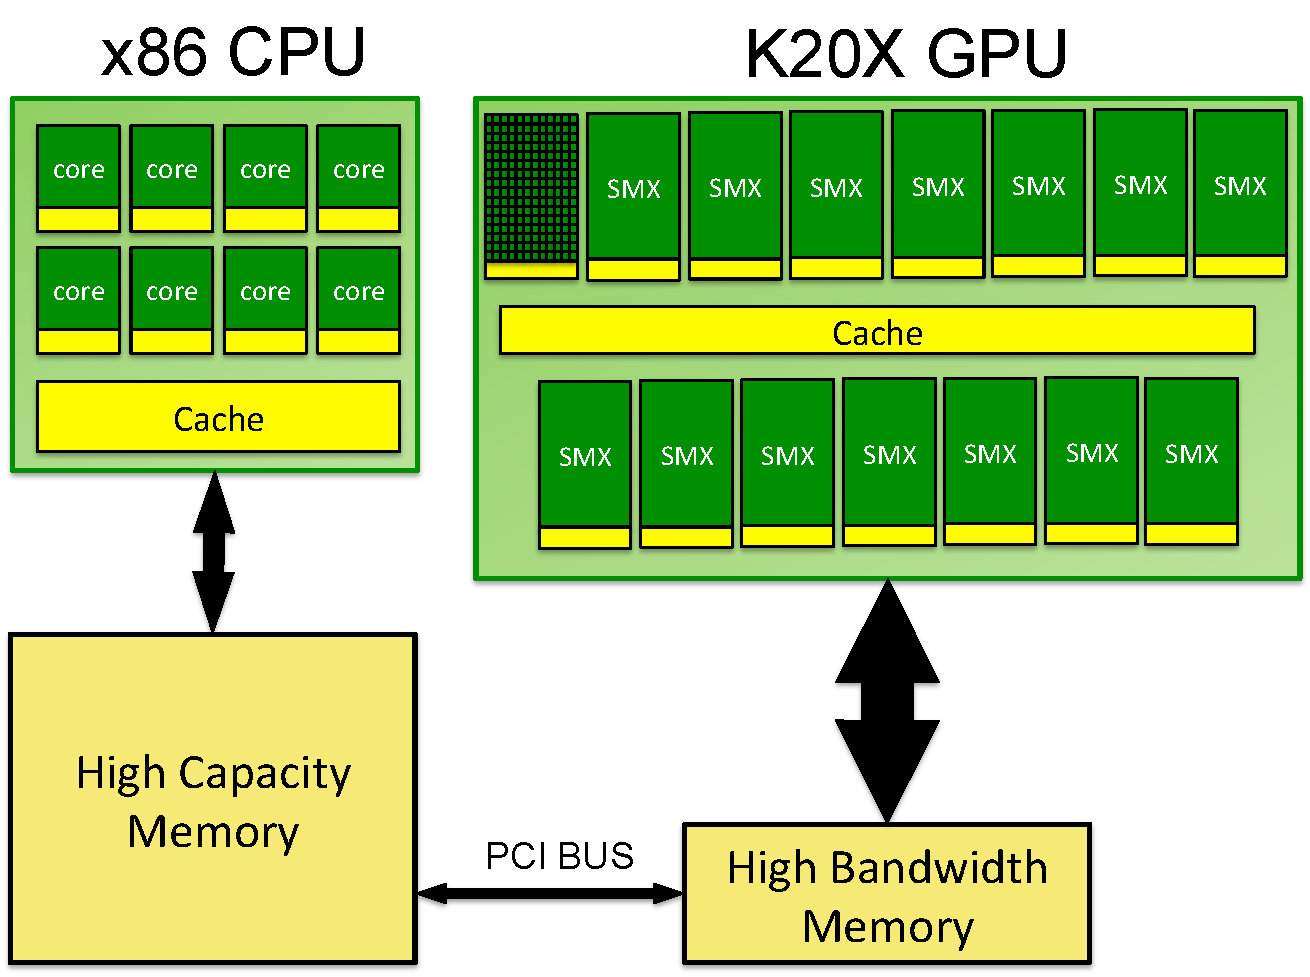
\includegraphics[width=0.9\textwidth]{./images/node.pdf}
    \end{center}
\end{frame}

%%%%%%%%%%%%%%%%%%%%%%%%%%%%%%%%%%%%
\begin{frame}[fragile]{}
%%%%%%%%%%%%%%%%%%%%%%%%%%%%%%%%%%%%
    \begin{info}{Host and device have separate memory spaces}
        \begin{itemize}
            \item data must be copied between host and device memory via PCI
            \item data must be in device memory for kernels to access
                \begin{itemize}
                    \item not strictly true\ldots
                    \item but a strict requirement for high performance in vast majority of cases (if you have to ask, it won't be good for you)
                \end{itemize}
            \item ensure data is in the right memory space \emph{before} computation starts
            \item on Piz Daint the respective bandwidths are:
            \begin{center}
            \begin{tabular}{lr}
                \textbf{host $\leftrightarrow$ device} & 6 GB/s \\
                \textbf{host memory} & 35 GB/s \\
                \textbf{device memory}  & 180 GB/s
            \end{tabular}
            \end{center}
        \end{itemize}
    \end{info}

\end{frame}

%%%%%%%%%%%%%%%%%%%%%%%%%%%%%%%%%%%%
\begin{frame}[fragile]{}
%%%%%%%%%%%%%%%%%%%%%%%%%%%%%%%%%%%%
    \begin{info}{CUDA uses C pointers to reference GPU memory}
        \centering \lst{double *data = // pass an address to either host or device memory}
        \begin{itemize}
            \item a pointer can hold an address in \emph{either} device \emph{or} host memory
            \begin{itemize}
                \item accessing a device pointer in host code, or vice versa, is \emph{undefined behaviour}
                \item we have to take care that we know which memory space a pointer is addressing
            \end{itemize}
            \item The CUDA runtime library provides functions that can be used to allocate, free and copy device memory
        \end{itemize}
    \end{info}

\end{frame}

%%%%%%%%%%%%%%%%%%%%%%%%%%%%%%%%%%%%
\begin{frame}[fragile]{}
%%%%%%%%%%%%%%%%%%%%%%%%%%%%%%%%%%%%
    \begin{info}{Allocating device memory}
        \centering \lst{cudaMalloc(void **ptr, size_t size)}
    \begin{itemize}
        \item \lst{size} number of bytes to allocate
        \item \lst{ptr} points to allocated memory on exit
    \end{itemize}
    \end{info}

    \begin{info}{Freeing device memory}
        \centering \lst{cudaFree(void *ptr)}
    \end{info}

    \begin{code}{Allocate memory for 100 doubles on device}
%..................................
        \begin{lstlisting}[style=boxcuda]
double *v; // C pointer that will point to device memory
auto size_in_bytes = 100*sizeof(double);
cudaMalloc(&v, size_in_bytes); // allocate memory
cudaFree(v);                   // free memory
\end{lstlisting}
%..................................
    \end{code}
\end{frame}

%%%%%%%%%%%%%%%%%%%%%%%%%%%%%%%%%%%%
\begin{frame}[fragile]{}
%%%%%%%%%%%%%%%%%%%%%%%%%%%%%%%%%%%%
    \begin{info}{Perform blocking copy (host waits for copy to finish)}
        \centering \lst{cudaMemcpy(void *dst, void *src, size_t size, cudaMemcpyKind kind)}
    \begin{itemize}
        \item \lst{dst} destination pointer
        \item \lst{src} source pointer
        \item \lst{size} number of \emph{bytes} to copy to \lst{dst}
        \item \lst{kind} enumerated type specifying \emph{direction} of copy:
            \\ one of
            \lst{cudaMemcpyHostToDevice}, \lst{cudaMemcpyDeviceToHost}, \lst{cudaMemcpyDeviceToDevice}, \lst{cudaMemcpyHostToHost}
    \end{itemize}
    \end{info}

    \begin{code}{Copy 100 doubles to device, then back to host}
%..................................
        \begin{lstlisting}[style=boxcuda]
int size = 100*sizeof(double); // size in bytes
double *v_d;
cudaMalloc(&v_d, size);              // allocate on device
double *v_h = (double*)malloc(size); // allocate on host
cudaMemcpy(v_d, v_h, size, cudaMemcpyHostToDevice);
cudaMemcpy(v_h, v_d, size, cudaMemcpyDeviceToHost);
\end{lstlisting}
%..................................
    \end{code}
\end{frame}

%%%%
\begin{frame}[fragile]{}

    \begin{info}{Errors happen\ldots}
        all API functions return error codes that indicate either:
        \begin{itemize}
            \item success
            \item an error in the API call
            \item an error in an earlier asynchronous call
        \end{itemize}
        the return value is the enum type \lst{cudaError_t}
        \begin{itemize}
            \item e.g. \lst{cudaError_t status = cudaMalloc(&v, 100);}
            \begin{itemize}
                \item status is \{\lst{cudaSuccess}, \lst{cudaErrorMemoryAllocation}\}
            \end{itemize}
        \end{itemize}
    \end{info}

    \begin{info}{Handling errors}
        \centering \lst{const char* cudaGetErrorString(status)}
        \begin{itemize}
            \item returns a string describing status
        \end{itemize}
        \centering \lst{cudaError_t cudaGetLastError()}
        \begin{itemize}
            \item returns the last error
            \item resets status to \lst{cudaSuccess}
        \end{itemize}
    \end{info}

\end{frame}

%%%%
\begin{frame}[fragile]{}

    \begin{code}{Copy 100 doubles to device \emph{with error checking}}
%..................................
        \begin{lstlisting}[style=boxcudatiny]
double *v_d;
int size = sizeof(double)*100;
double *v_host = (double*)malloc(size);
cudaError_t status;

status = cudaMalloc(&v_d, size);
if(status != cudaSuccess) {
  printf("cuda error : %s\n", cudaGetErrorString(status));
  exit(1);
}

status = cudaMemcpy(v_d, v_h, size, cudaMemcpyHostToDevice);
if(status != cudaSuccess) {
  printf("cuda error : %s\n", cudaGetErrorString(status));
  exit(1);
}
        \end{lstlisting}
%..................................
    \end{code}

    \begin{info}{It is essential to test for errors}
        But it is tedious and obfuscates our source code if it is done in line for every API and kernel call\ldots
    \end{info}
\end{frame}

%%%%%%%%%%%%%%%%%%%%%%%%%%%%%%%%%%%%%%%%%%%%
\begin{frame}[fragile]{Exercise: API Basics}
%%%%%%%%%%%%%%%%%%%%%%%%%%%%%%%%%%%%%%%%%%%%
    Open \lst{cuda/exercises/axpy/util.h}
    \begin{enumerate}
        \item what does \lst{cuda_check_error()} do?
        \item look at the template wrappers \lst{malloc_host} \& \lst{malloc_device}
        \begin{itemize}
            \item what do they do?
            \item what are the benefits over using \lst{cudaMalloc} and \lst{free} directly?
            \item do we need corresponding functions for \lst{cudaFree} and \lst{free}?
        \end{itemize}

        \item write a wrapper around \lst{cudaMemcpy} for copying data \texttt{host$\rightarrow$device} \& \texttt{device$\rightarrow$host}
        \begin{itemize}
            \item remember to check for errors!
        \end{itemize}

        \item compile the test and run
        \begin{itemize}
            \item it will pass with no errors on success
        \end{itemize}

    \vspace{-5pt}
\begin{lstlisting}[style=terminal]
make axpy_cublas
aprun ./axpy_cublas 8
\end{lstlisting}
    \end{enumerate}

\end{frame}

